% === T14 - Compilador, Ensamblador y Linker ===
% David Alejandro Gonzalez Marquez
% fokerman@gmail.com
% https://github.com/fokerman/computingSystemsCourse

\documentclass[aspectratio=169]{beamer}
% \documentclass[aspectratio=169, handout]{beamer}

% % % Packages
\usepackage[sfdefault]{AlegreyaSans}
\usepackage{inconsolata}
\usepackage{multicol}
\usepackage{multirow}
\usepackage[spanish]{babel}
\usepackage[utf8]{inputenc}
\usepackage{enumerate}
\usepackage{color}
\usepackage{xcolor}
\usepackage[absolute,overlay]{textpos}
  \setlength{\TPHorizModule}{1mm}
  \setlength{\TPVertModule}{1mm}
\usepackage{framed}
\usepackage{mfirstuc} % para poner en mayusculas la primer letra
\usepackage{xspace} % para crear espacios en comandos 
\usepackage{pbox}
\usepackage{tikz}
\usepackage{mathabx}
\usepackage{colortbl}
\usepackage{ulem} % para tener tachado

% % % Beamer config
\usetheme{Pittsburgh}
\usecolortheme[rgb={1,0.48,0.0}]{structure}
\setbeamercolor{block title}{fg=white,bg=verdeuca}
\xdefinecolor{verdeuca}{rgb}{0.0,0.48,0.54}
\xdefinecolor{naranjauca}{rgb}{1,0.48,0.0}
\setbeamercolor{palette quaternary}{fg=white,bg=verdeuca}
\setbeamertemplate{title page}[default][colsep=-4bp, rounded=true] % remove title shadow
\setbeamertemplate{frametitle}[default][colsep=-2bp, shadow=false] % remove frame title shadow
\setbeamertemplate{navigation symbols}{} % remove navigation symbols
\beamertemplatenavigationsymbolsempty

% % % Colors
\definecolor{AzulClaro}{rgb}{.31,.506,.741}
\definecolor{Gris}{gray}{0.8}
\definecolor{Celeste}{rgb}{.255,.41,.884}
\definecolor{Rojo}{rgb}{1, 0, 0}
\definecolor{a}{rgb}{0.0, 0.53, 0.74}
\definecolor{r}{rgb}{0.89, 0.0, 0.13}
\definecolor{v}{rgb}{0.0, 0.5, 0.0}
\definecolor{y}{rgb}{0.0, 0.5, 0.5}
\definecolor{rojo}{HTML}{F1521B}
\definecolor{verde}{HTML}{80CD29}
\definecolor{amarillo}{HTML}{FABC09}
\definecolor{azul}{HTML}{00ADF1}

% % % Rename
\newcommand{\tab}[0]{\hspace{15pt}}

% % % Blocks
\setbeamercolor{block body}{fg=black, bg=black!10}
\setbeamercolor{block title}{fg=black, bg=black!20}
\setbeamercolor{coloredboxstuffNaranja}{fg=naranjauca,bg=black!10} %% PARA LOS BOX
\setbeamercolor{coloredboxstuffVerde}{fg=verdeuca,bg=black!10} %% PARA LOS BOX

% % % Special Packages
\usepackage{fontawesome}
\usepackage{pgf}

\usepackage{array}
\newcommand{\PreserveBackslash}[1]{\let\temp=\\#1\let\\=\temp}
\newcolumntype{C}[1]{>{\PreserveBackslash\centering}p{#1}}
\newcolumntype{R}[1]{>{\PreserveBackslash\raggedleft}p{#1}}
\newcolumntype{L}[1]{>{\PreserveBackslash\raggedright}p{#1}}

% % % Start

\title{\Huge Compilador, Ensamblador y Linker}
% \subtitle{}
\author{David Alejandro González Márquez}
\input{../university}
\date{}

\begin{document}

\begin{frame}[plain]
    \titlepage
    \begin{textblock}{140}(10,70)
    \textcolor{rojo}{
    \textbf{Atención}: La clase será grabada por el anfitrión para su posterior y eventual uso académico dentro de nuestra institución. Su participación en la clase implica brindar su consentimiento para participar en la grabación, aunque pueden mantener su video apagado.}
    \end{textblock}
\end{frame}

\begin{frame}[fragile,t]{Lenguajes}
    \textcolor{naranjauca}{Compilados}\\
    El código se transforma a código nativo de la plataforma. Para esto debe ser compilado, ensamblado y linkeado. El resultado es un \textbf{archivo binario ejecutable} que el sistema operativo entiende cómo cargar para poder ejecutar.\\
    \textcolor{gray}{Ejemplos: C, C++, C\#, Go}\\
    \vspace{0.2cm}
    \pause
    \textcolor{naranjauca}{Interpretados}\\
    El código es \textbf{leído e interpretado} como instrucciones o comandos. El programa que realiza esta acción es el intérprete.\\ 
    \textcolor{gray}{Ejemplos: Python, Ruby, JavaScript, PHP}\\
    \vspace{0.2cm}
    \pause
    \textcolor{naranjauca}{Código intermedio}\\
    El código es transformado a \texttt{bytecode} y ejecutado por una \textbf{máquina virtual}. Este código puede ser utilizado en múltiples plataformas. Cuentan con \texttt{JIT} (Just-In-Time Compiler) que consiste en transformar el \texttt{bytecode} a código de máquina nativo.\\
    \textcolor{gray}{Ejemplos: Java, Scala, Groovy}\\
\end{frame}

\begin{frame}[fragile,t]{Compilador}
    El \textbf{compilador} es un programa que traduce código en un lenguaje de programación a código en otro lenguaje de programación, generalmente lenguaje ensamblador.\\
    \begin{center}
    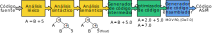
\includegraphics[scale=0.6]{img/compiladorEtapas.pdf}
    \end{center}
    El código pasa por diferentes etapas hasta generar instrucciones de ensamblador.\\
    \bigskip
    \pause
    En algunos lenguajes, existen procesos anteriores al compilador,\\
    como el \textbf{precompilador} o la resolución de \textbf{macros}.\\
    \bigskip
    \pause
    En la etapa de \textbf{optimización} el código es transformado para realizar la misma acción pero de forma diferente a la escrita por el programador, potencialmente obteniendo mejor rendimiento.
    % - Código fuente
    % - Analisis léxico
    % - Analisis sintáctico
    % - Analisis semántico
    % - Generación de código intermedio
    % - Optimización de código
    % - Generación de código ejecutable
    % - Ensamblado
\end{frame}

\begin{frame}[fragile,t]{Ensamblador}
    El \textbf{ensamblador} transforma instrucciones ASM en código binario (código objeto).\\
    \bigskip
    \pause
    Esta transformación es directa, no requiere interpretar qué acciones realiza el programa.\\
    \bigskip
    \pause
    Cuenta con \textbf{pseudoinstrucciones} que le indican al ensamblador cómo proceder para generar código o datos.
    El archivo objeto resultante es compatible solo con la arquitectura destino.\\
    \bigskip
    \pause
    \begin{block}{Archivo objeto}
    Se puede ver como código binario con faltantes e información adicional.\\
    \vspace{0.2cm}
    $\rightarrow$ Los faltantes son funciones o procedimientos no registrados en el archivo fuente.\\
    \vspace{0.2cm}
    $\rightarrow$ La información adicional es una \textbf{tabla de símbolos}, con todos los símbolos declarados en el archivo objeto, y todos los faltantes con su nombre y dirección relativa.
    \end{block}
\end{frame}

\begin{frame}[fragile,t]{Tabla de símbolos}
    A medida que se construye un programa se \textbf{genera una tabla con \emph{símbolos}}.\\
    \bigskip
    Llamamos símbolo a un \textbf{nombre} asociado a un \textbf{valor} numérico entero.\\
    Cada símbolo puede estar definido (T) o no definido (U), entre otros estados.\\
    \bigskip
    Los símbolos asocian nombres a direcciones de memoria \textbf{relativas}\\ dentro de un segmento del archivo objeto.\\
    \pause
    \bigskip
    \textcolor{gray}{Ejemplo: Símbolos dentro de un archivo objeto.}
    { \small
    \begin{verbatim}
    0000000000000000 T addFirst
                     U free
                     U _GLOBAL_OFFSET_TABLE_
    00000000000000d1 T main
                     U malloc
    000000000000003c T removeLast
    \end{verbatim} }
    \begin{textblock}{100}(100,75)
    \only<2->{
    \textcolor{verdeuca}{Comando útil}\\
    \textbf{nm}: Mostrar tabla de símbolos.
    }
    \end{textblock}
\end{frame}

\begin{frame}[fragile,t]{Linker}
    \begin{textblock}{64}(10,15)
    El \textbf{Linker} se encarga de tomar un conjunto de archivos objeto y enlazarlos en uno solo.\\
    \bigskip
    Resuelve todas las \textbf{dependencias} entre archivos, con el sistema y con bibliotecas externas de funciones.\\
    \bigskip
    El resultado es un \textbf{programa ejecutable} para un sistema operativo particular.\\
    \end{textblock}
    \begin{textblock}{100}(80,7) \only<4->{\includegraphics[scale=0.7]{img/linker-layer3.pdf}} \end{textblock}
    \begin{textblock}{100}(80,7) \only<5->{\includegraphics[scale=0.7]{img/linker-layer4.pdf}} \end{textblock}
    \begin{textblock}{100}(80,7) \only<6->{\includegraphics[scale=0.7]{img/linker-layer5.pdf}} \end{textblock}
    \begin{textblock}{100}(80,7) \only<7->{\includegraphics[scale=0.7]{img/linker-layer6.pdf}} \end{textblock}
    \begin{textblock}{100}(80,7) \only<2->{\includegraphics[scale=0.7]{img/linker-layer1.pdf}} \end{textblock}
    \begin{textblock}{100}(80,7) \only<3->{\includegraphics[scale=0.7]{img/linker-layer2.pdf}} \end{textblock}
    \begin{textblock}{100}(10,73)
    \only<8->{
    \textcolor{verdeuca}{Comando útil}\\
    \textbf{ldd}: Mostrar bibliotecas compartidas\\ (\emph{shared libraries})
    }
    \end{textblock}
\end{frame}

\begin{frame}[fragile,t]{Static vs Dynamic Linker}
    Las aplicaciones utilizan \textbf{bibliotecas} (\emph{library}) de funciones externas. Ejemplo: \texttt{libc}.\\
    Estas pueden estar enlazadas de forma estática o dinámica.\\
    \pause
    \vspace{0.2cm}
    \textcolor{naranjauca}{Enlazado estático}\\
    Se resuelve en tiempo de enlazado o linkeo: todo el código de la biblioteca forma parte del binario resultante.
    Existirán múltiples copias del mismo código en memoria para cada aplicación.
    \begin{center}
    \includegraphics[scale=0.5]{img/static-dynamic-link-layer1.pdf}
    \end{center}
    \pause
    \textcolor{naranjauca}{Enlazado dinámico}\\
    Se resuelve en tiempo de ejecución: el código de la biblioteca no forma parte del binario.
    Existe solo una copia de la biblioteca que es usada por múltiples aplicaciones.
    \begin{center}
    \includegraphics[scale=0.5]{img/static-dynamic-link-layer2.pdf}
    \end{center}
    
\end{frame}

% \begin{frame}[fragile,t]{Position-Independent Code}
% % position-independent code PIC
% % position-independent executable PIE
% ...
% \end{frame}

\begin{frame}[fragile,t]{Niveles de optimización}
La optimización de código se encarga transformar el código intermedio en una nueva versión que mejore alguna característica particular:
%    Options That Control Optimization
%        These options control various sorts of optimizations.
%        Without any optimization option, the compiler's goal is to reduce the cost of compilation and to make debugging produce the expected results.  Statements are independent: if you stop the program with a breakpoint between
%        statements, you can then assign a new value to any variable or change the program counter to any other statement in the function and get exactly the results you expect from the source code.
%        Turning on optimization flags makes the compiler attempt to improve the performance and/or code size at the expense of compilation time and possibly the ability to debug the program.
%        The compiler performs optimization based on the knowledge it has of the program.  Compiling multiple files at once to a single output file mode allows the compiler to use information gained from all of the files when
%        compiling each of them.
%        Not all optimizations are controlled directly by a flag.  Only optimizations that have a flag are listed in this section.
%        Most optimizations are completely disabled at -O0 or if an -O level is not set on the command line, even if individual optimization flags are specified.  Similarly, -Og suppresses many optimization passes.
%        Depending on the target and how GCC was configured, a slightly different set of optimizations may be enabled at each -O level than those listed here.  You can invoke GCC with -Q --help=optimizers to find out the exact set of
%        optimizations that are enabled at each level.
\vspace{0.2cm}
\begin{itemize}
\setlength\itemsep{0.5cm}
\item[-O0] Reduce el tiempo de compilación y permite obtener resultados correctos del debugger.
% Reduce compilation time and make debugging produce the expected results.  This is the default.
\item[-O1] Optimiza el costo de ejecución y el tamaño del código, no realiza optimizaciones que demoren mucho tiempo.
%             Optimize. 
%             Optimizing compilation takes somewhat more time, and a lot more memory for a large function.
%             With -O, the compiler tries to reduce code size and execution time, without performing any optimizations that take a great deal of compilation time.
%            -O turns on the following optimization flags:
%            -fauto-inc-dec -fbranch-count-reg -fcombine-stack-adjustments -fcompare-elim -fcprop-registers -fdce -fdefer-pop -fdelayed-branch -fdse -fforward-propagate -fguess-branch-probability -fif-conversion -fif-conversion2
%            -finline-functions-called-once -fipa-profile -fipa-pure-const -fipa-reference -fipa-reference-addressable -fmerge-constants -fmove-loop-invariants -fomit-frame-pointer -freorder-blocks -fshrink-wrap -fshrink-wrap-separate
%            -fsplit-wide-types -fssa-backprop -fssa-phiopt -ftree-bit-ccp -ftree-ccp -ftree-ch -ftree-coalesce-vars -ftree-copy-prop -ftree-dce -ftree-dominator-opts -ftree-dse -ftree-forwprop -ftree-fre -ftree-phiprop -ftree-pta
%            -ftree-scev-cprop -ftree-sink -ftree-slsr -ftree-sra -ftree-ter -funit-at-a-time
\item[-O2] Optimiza más. Agrega todas las optimizaciones, excepto las que compiten con el tamaño del código y el tiempo de ejecución.
%             Optimize even more.  GCC performs nearly all supported optimizations that do not involve a space-speed tradeoff.  As compared to -O, this option increases both compilation time and the performance of the generated code.
%            -O2 turns on all optimization flags specified by -O.  It also turns on the following optimization flags:
%            -falign-functions  -falign-jumps -falign-labels  -falign-loops -fcaller-saves -fcode-hoisting -fcrossjumping -fcse-follow-jumps  -fcse-skip-blocks -fdelete-null-pointer-checks -fdevirtualize  -fdevirtualize-speculatively
%            -fexpensive-optimizations -fgcse  -fgcse-lm -fhoist-adjacent-loads -finline-small-functions -findirect-inlining -fipa-bit-cp  -fipa-cp  -fipa-icf -fipa-ra  -fipa-sra  -fipa-vrp -fisolate-erroneous-paths-dereference
%            -flra-remat -foptimize-sibling-calls -foptimize-strlen -fpartial-inlining -fpeephole2 -freorder-blocks-algorithm=stc -freorder-blocks-and-partition  -freorder-functions -frerun-cse-after-loop -fschedule-insns
%            -fschedule-insns2 -fsched-interblock  -fsched-spec -fstore-merging -fstrict-aliasing -fthread-jumps -ftree-builtin-call-dce -ftree-pre -ftree-switch-conversion  -ftree-tail-merge -ftree-vrp
%            Please note the warning under -fgcse about invoking -O2 on programs that use computed gotos.
%            NOTE: In Ubuntu 8.10 and later versions, -D_FORTIFY_SOURCE=2 is set by default, and is activated when -O is set to 2 or higher.  This enables additional compile-time and run-time checks for several libc functions.  To
%            disable, specify either -U_FORTIFY_SOURCE or -D_FORTIFY_SOURCE=0.
\item[-O3] Optimiza más aún. Agrega todas las optimizaciones.
%            Optimize yet more.  -O3 turns on all optimizations specified by -O2 and also turns on the following optimization flags:
%            -fgcse-after-reload -finline-functions -fipa-cp-clone -floop-interchange -floop-unroll-and-jam -fpeel-loops -fpredictive-commoning -fsplit-paths -ftree-loop-distribute-patterns -ftree-loop-distribution
%            -ftree-loop-vectorize -ftree-partial-pre -ftree-slp-vectorize -funswitch-loops -fvect-cost-model -fversion-loops-for-strides
\item[-Os] Optimiza el tamaño del ejecutable.
%             Optimize for size.  -Os enables all -O2 optimizations except those that often increase code size:
%            -falign-functions  -falign-jumps -falign-labels  -falign-loops -fprefetch-loop-arrays  -freorder-blocks-algorithm=stc
%            It also enables -finline-functions, causes the compiler to tune for code size rather than execution speed, and performs further optimizations designed to reduce code size.
% \item[-Ofast]
%            Disregard strict standards compliance.  -Ofast enables all -O3 optimizations.  It also enables optimizations that are not valid for all standard-compliant programs.  It turns on -ffast-math and the Fortran-specific
%            -fstack-arrays, unless -fmax-stack-var-size is specified, and -fno-protect-parens.
% \item[-Og] Optimize debugging experience.  -Og should be the optimization level of choice for the standard edit-compile-debug cycle, offering a reasonable level of optimization while maintaining fast compilation and a good debugging
%            experience.  It is a better choice than -O0 for producing debuggable code because some compiler passes that collect debug information are disabled at -O0.
%            Like -O0, -Og completely disables a number of optimization passes so that individual options controlling them have no effect.  Otherwise -Og enables all -O1 optimization flags except for those that may interfere with
%            debugging:
 
\end{itemize}
\end{frame}

\begin{frame}[fragile,t]{Información de debug}
    El código cuando es cargado consiste en solo instrucciones y datos.\\
    \bigskip
    Para \textbf{entender} el flujo del programa y su relación con el código fuente,\\
    es necesario que al momento de compilación se \textbf{genere información de \emph{debug}},\\
    y que esta información se preserve durante todo el proceso de generación de código.\\
    \bigskip
    \pause
    \textcolor{gray}{Ejemplo: Archivo ASM con información de debugging.}
    { \small
    \begin{verbatim}
    addFirst:
    .LFB6:
        .file 1 "lista.c"
        .loc 1 9 49
        .cfi_startproc
        endbr64
        pushq %rbp
        .cfi_def_cfa_offset 16
        .cfi_offset 6, -16
        movq %rsp, %rbp
    \end{verbatim} }
\end{frame}

% \begin{frame}[fragile,t]{Formatos de programas ejecutables}
% - elf
% - exe
% - com
% \end{frame}

\begin{frame}[fragile,t]{Compilar, Ensamblar y Enlazar en C}
    \begin{textblock}{60}(10,15)
    \textcolor{naranjauca}{Compilar}\\
    \texttt{\$ gcc -S -o lista.s lista.c}\\
    \bigskip
    \textcolor{naranjauca}{Ensamblar}\\
    \texttt{\$ gcc -c -o lista.o lista.c}\\ % \texttt{\$ as -o lista.o lista.s}\\
    \bigskip
    \textcolor{naranjauca}{Enlazar}\\
    \texttt{\$ gcc -o lista.out lista.c}\\
    \end{textblock}
    \begin{textblock}{100}(70,7)
     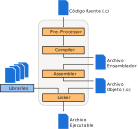
\includegraphics[scale=0.6]{img/compilacionC.pdf}
    \end{textblock}
\end{frame}

% \begin{frame}[fragile,t]{Herramientas en Linux}
% nm
% ldd
% objdump
% \end{frame}

\begin{frame}[fragile]
    \frametitle{Bibliografía}
    \begin{itemize}
     \setlength\itemsep{0.5cm}
    \item[-] \small Tanenbaum, “Organización de Computadoras. Un Enfoque Estructurado”, 4ta Edición, 2000.\\
    \begin{itemize}
     \item \textbf{Capitulo 7 - El nivel de lenguaje ensamblado}
     \begin{itemize} 
        \item 7.3 El proceso de ensamblado
        \item 7.4 Enlazado y carga
     \end{itemize}
    \end{itemize}
    \item[-] \small Null, “Essentials of Computer Organization and Architecture”, 5th Edition, 2018.\\
    \begin{itemize}
    \item \textbf{Chapter 8 - System Software}
     \begin{itemize} 
        \item 8.4.1 Assemblers and Assembly
        \item 8.4.2 Link Editors
        \item 8.4.3 Dynamic Link Libraries
        \item 8.4.4 Compilers
        \item 8.4.5 Interpreters
     \end{itemize}
    \end{itemize}
%     \item[-] \small Silberschatz, “Fundamentos de Sistemas Operativos”, 7ma Edición, 2006.\\
%     \item[-] \small Tanenbaum, “Modern Operating Systems”, 4th Edition, 2015.\\
    \end{itemize}
\end{frame}

\begin{frame}[plain]
    \begin{center}
    \vspace{2cm}
    \huge ¡Gracias!\\
    \vspace{2cm}
    \normalsize Recuerden leer los comentarios adjuntos\\ en cada clase por aclaraciones.
    \end{center}
\end{frame}

\end{document}

% % % % % % % % % % % % % % % % % % 
% EJEMPLOS:

\begin{frame}[fragile]
    \frametitle{Bla}
    \begin{itemize}
    \item[-] Bla bla \textbf{ble} bla bla
    \item[-] Bla bla \textbf{ble} bla bla
    \end{itemize}
\end{frame}

\begin{frame}[fragile]
    \frametitle{Bla}
    \begin{block}{\texttt{BLA}}
    Bla Bla
    \end{block}
    \begin{multicols}{2}
    \begin{tabular}{ll}
    la & la \\
    \end{tabular}
    \columnbreak
    \begin{tabular}{ll}
    la & la \\
    \end{tabular}
    \end{multicols}
\end{frame}

\begin{frame}
    \frametitle{Bla}
    \begin{itemize}
    \item Bla bla
    \begin{center}
    \includegraphics[scale=0.7]{img/struct_aling.pdf}
    \end{center}
    Bla bla
    \end{itemize}
\end{frame}

\begin{frame}[fragile]
    \frametitle{Bla}
%     \begin{textblock}{100}(10,10)
%     Bla
%     \end{textblock}
\end{frame}
